\documentclass{article}
\usepackage{graphicx}
\graphicspath{ {./Screenshots/} }
\title{ Multilayer Neural Networks and Back Propagation : Project - 2}
\author{Atsushi oba (s1230128),        Hitoshi Ikuta (m5221106) \\
  \and Chowdhury Md Intisar (m5212106),        Yunosuke Teshima (m5221151)
}

\begin{document}
\maketitle
\section{Back Propagation Algorithm}
In this project, we have implemented the Back propagation learning algorithm to
solved the 4-bit parity problem. The basic property of back propagation is, it
propagates the error from its output layer to the subsequent hidden layer. The
weight of the network is updated by gradient descent method. 

Below is a figure of 3 layer neural network 
\begin{figure}[h]
 \caption{A 3-layer Neural Network}
 \centering
  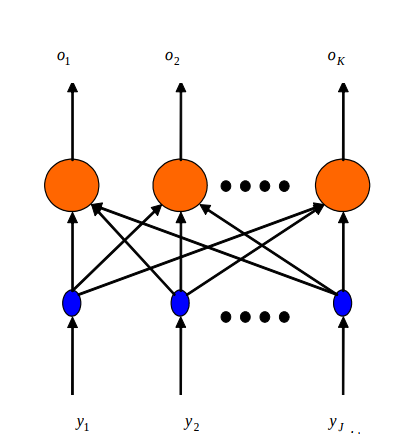
\includegraphics[width=5cm, height=5cm]{Network.png}
\end{figure}
 
\section{Terms and Terminology}
\begin{itemize}
  \item  \( z_{ i}\) is the i-th input
  \item  \(y_{j}\) is the output of the j-th neuron
  \item  \(o_{k}\) is the weight from the i-th input to the j-th hidden neuron
  \item  \(v_{ji}\) is the weight from the i-th input to the j-th hidden neuron
  \item  \(w_{kj}\) is the weight from the j-th hidden neuron to the k-th output neuron
\end{itemize}

\section{Rule for Updating weights}
The rule for updating the weight is same as the previous project-1 for output
layer. However, the rule for hidden layer weight update has few changes as
follows. 
For the hidden layer 
\begin{equation}
  \(v_{ji} = v_{ji}^{old} + \eta\delta_{yj}z_{i}\)
\end{equation}

Thus we require to calcualte the deltas of the neuron. Following two equation
was used to calculate the delta for output and hidden layer respectively.
\begin{equation}
  \(\delta_{ok} = (d_k - o_k)(1-o_{k}^2)/2\)
\end{equation}

\begin{equation}
  \(\delta_{yj}= \Big(\sum_{k=1}^{K} \delta_{ok}W_{kj} \Big) (1-y_{j}^{2})/2 \)
\end{equation}

The above two equations are derived from the error function with the method of
chain rule. 

\section{Input and Output Generations}
First, we have written an algorithm to generated all possible 4 bit
configurations for parity. Next, we have generated output based on the even and
odd occurrence of 1 in the 4 bit parity as follows. 
\begin{figure}[h]
 \caption{Input generate by recursive function}
 \centering
  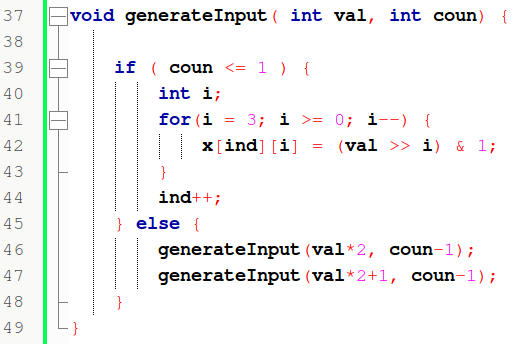
\includegraphics[width=5cm, height=5cm]{GenerateInput.png}
\end{figure}
 
\begin{figure}[h]
 \caption{Generate Output}
 \centering
  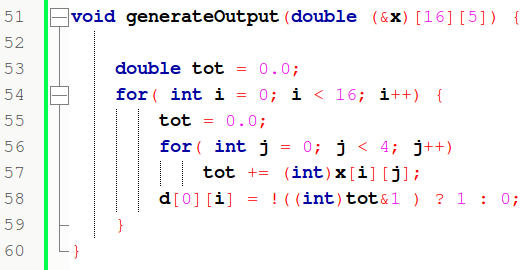
\includegraphics[width=5cm, height=5cm]{GenerateOutput.png}
\end{figure}

 
\begin{figure}[h]
 \caption{Output of the program}
 \centering
  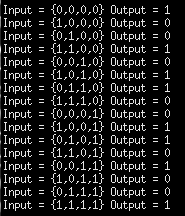
\includegraphics[width=5cm, height=5cm]{InputOutput.png}
\end{figure}




\section{Results}
The network has been tested with different number of neuron ranging from 4 to
10. Each run with different number of neuron gave different result. The result
has been depicted below.

\begin{table}
  \label{table:table1}
  \begin{center}
    \caption{No. of Neuron and Epochs}
    \begin{tabular}{l|c}
     \textbf{Neurons} & \textbf{Epochs}\\
      \hline
      4  & 52496\\
      5  & 35741\\
      6  & 9676\\
      7  & 9757\\
      8  & 9603\\
      9  & 10769\\
      10 & 8999\\
    \end{tabular}
  \end{center}
\end{table}

As we can see from Table 1, with increase of hidden neuron the
number of epoch also decreases. But, sometimes use of too many hidden neuron
can result in over-fitting. One key point of observation is, the epoch for
6,7,8 is nearly same.

Thus, we can conclude that 
\begin{itemize}
   \item With the increase of neuron in the hidden layer complex function can
    be constructed.
  \item Hidden layer is necessary if we want to solve a non-linear problem.
  \item As the number of neuron in hidden layer was increased it took less
    epochs to converge to solution.
  \item Care should be taken in case,  increase number of neuron can cause over
    fitting problem.  
  \item Too many neuron in hidden layer / or too many hidden layer is
    computationally expensive. Thus, a trade off is to be made in choosing
    number    of neuron and compromising performance. 
\end{itemize}
\end{document}
